\documentclass{beamer}
\usepackage[utf8]{inputenc}

%fonts
%\usepackage{bookman}
%\usepackage{utopia} 
%\usepackage{tgbonum}
%\usepackage{mathptmx}
\usepackage{multirow}
\usetheme{Madrid}
\usepackage{graphics}
%\usefonttheme{structuresmallcapsserif}
%\usefonttheme{serif}
%\usefonttheme{default}

%\usecolortheme{whale}
%\usecolortheme{orchid}
%\usecolortheme{beaver}
%\usecolortheme{default}

\useinnertheme{rectangles}
%\useoutertheme{infolines}
\newcommand{\revision}[1]{\textcolor{black}{#1}}
\newcommand{\revisiondel}[1]{}
\newcommand{\src}{\ensuremath{\mathbf{f}}} % source sentence
\newcommand{\trg}{\ensuremath{\mathbf{e}}} % target sentence
\newcommand{\domain}[1]{\texttt{\textsc{#1}}}
\newcommand{\system}[1]{\texttt{{#1}}}
\newcommand{\vlambda}{\ensuremath{\boldsymbol\lambda}\xspace} %
\newcommand{\soft}[1]{\texttt{\textit{#1}}}
\usepackage[draft]{todo}
\newcommand{\fyTodo}[1]{\Todo[FY:]{\textcolor{orange}{#1}}}
\newcommand{\fyTodostar}[1]{\Todo*[FY:]{\textcolor{orange}{#1}}}
\newcommand{\fyDone}[1]{\done[FY]\Todo[FY:]{\textcolor{orange}{#1}}}
\newcommand{\fyDonestar}[1]{\done[FY]\Todo[FY:]{\textcolor{orange}{#1}}}
\usepackage{enumitem}
\setlist[itemize,1]{label=$\star$}
\setlist[itemize,2]{label=$\bullet$}
%------------------------------------------------------------
%This block of code defines the information to appear in the Title page
\title[Revisiting multi-domain NMT] %optional
{
    {\large Revisiting multi-domain neural machine translation}
}
\author[MinhQuang Pham] % (optional)
{
    MinhQuang Pham\inst{\dag\ddag},
    Josep Crego\inst{\dag},
    Fran\c cois Yvon\inst{\ddag}
}
\institute[SYSTRAN] % (optional)
{
    \inst{\dag} SYSTRAN, 5 rue Feydeau, 75002, Paris, France \and
    \vspace{-0.2cm}
    \inst{\ddag} Universit\'e Paris-Saclay, CNRS, LISN, 91400, Orsay, France \\
    \vspace{0.5cm}
    
\includegraphics[height=1.0cm]{systran-logo.png}
    
\includegraphics[height=1.0cm]{cnrs-logo.png}
%    
\includegraphics[height=1.0cm]{limsi-logo.png}
    
\includegraphics[height=1.0cm]{ups-logo.png}
    \vspace{1.5cm}
}
\date[EACL'2021] % (optional)
{
    {\footnotesize \textsc{}}
}
%\logo{
%
\includegraphics[height=1.0cm]{systran-logo.png}
%
\includegraphics[height=1.0cm]{limsi-logo.png}
%}
%End of title page configuration block
%------------------------------------------------------------



%------------------------------------------------------------
%The next block of commands puts the table of contents at the 
%beginning of each section and highlights the current section:
\AtBeginSection[]
{
  \begin{frame}
    \frametitle{Table of Contents} 
    \tableofcontents[currentsection]
  \end{frame}
}
%------------------------------------------------------------

\begin{document}

%The next statement creates the title page.
\frame{\titlepage}

%---------------------------------------------------------
%This block of code is for the table of contents after
%the title page
\begin{frame}
\frametitle{Table of Contents}
\tableofcontents
\end{frame}
%---------------------------------------------------------


%%%%%%%%%%%%%%%%%%%%%%%%%%%%%%%%%%%%%%%%%%%%%%%%%%%%%%%%%%
\section{Introduction} %%%%%%%%%%%%%%%%%%%%%%%%%%%%%%%%%%%
%%%%%%%%%%%%%%%%%%%%%%%%%%%%%%%%%%%%%%%%%%%%%%%%%%%%%%%%%%

%---------------------------------------------------------
\begin{frame}
\frametitle{Multi-domain NMT}
\centering
\begin{itemize}
	\item<1-> Text resources are highly variable in terms of domains
	\begin{itemize}
		\item<2-> Horizontally.
		\begin{itemize}
			\item<3-> OPUS corpora: $\sim$ 30 domains.
			\item<4-> Client data: $\sim$ one domain.
		\end{itemize}
		\item<5-> Vertically
		\begin{itemize}
			\item<6-> Economic domain: banking text (ECB), economic press (EESC), financial text (client corpora).
		\end{itemize}
	\end{itemize}
	\item<7-> Unbalanced training data
	\begin{itemize}
		\item<8-> Low-resource domains: religion, tourism, talks.
		\item<9-> High-resource domains: law, medical.
	\end{itemize}
	\item<10-> Trade-off between specialization and generalization
	\item<11-> Catastrophic forgetting. 
	\item<12-> Large size of fine-tuned models
		\begin{itemize}
		\item<13-> 1 Gb/ Transformer model.
		\end{itemize} 
	\item<14-> Unknown domain
		\begin{itemize}
		\item<15-> In training phase $\sim$ incremental learning.
		\item<16-> In testing phase $\sim$ robustness.
		\end{itemize}
\end{itemize}
\end{frame}
%---------------------------------------------------------


%---------------------------------------------------------
\begin{frame}
\frametitle{Axiomatic of multi-domain NMT}

\begin{itemize}
\item<1-> Required properties:
	\begin{itemize}
		\item<2-> Robustness to unbalanced data.
		\item<3-> Robustness to new domain.
		\item<4-> Ability to learn from other domain.
		\item<5-> Ability to handle unlabeled training data (eg via clustering).
		\item<6-> Ability to perform continuous learning.
	\end{itemize}
\item<7-> Multi-criteria evaluation:
	\begin{itemize}
		\item<8-> Variable-size in-domain corpora in training data.
		\item<9-> In-domain and out-domain test sets. 
		\item<10-> Fuzzy domain separation.
		\item<11-> Training in considering unsupervised clusters as domains.
		\item<12-> Continuation of training with new domain data.
	\end{itemize}
\end{itemize}

\end{frame}
%---------------------------------------------------------


%%%%%%%%%%%%%%%%%%%%%%%%%%%%%%%%%%%%%%%%%%%%%%%%%%%%%%%%%%
\section{Experimental setting} %%%%%%%%%%%%%%
%%%%%%%%%%%%%%%%%%%%%%%%%%%%%%%%%%%%%%%%%%%%%%%%%%%%%%%%%%

%---------------------------------------------------------
\begin{frame}
\frametitle{Revisited methods}
\begin{itemize}
	\item<1-> Domain control (Kobus et al 2017)
	\begin{itemize}
		\item<2-> Domain tag (DC-Tag)
		\item<3-> Domain embedding (DC-Feat)
	\end{itemize}
	\item<4-> Lexicalized Domain Representation (Pham et al 2019) (LDR)
	\item<5-> Domain mixing (Britz et al 2018)
	\begin{itemize}
		\item<6-> Domain tag in target TTM)
		\item<7-> Domain mixing (DM)
		\item<8-> Adversarial Domain mixing (ADM)
	\end{itemize}
	\item<9-> Residual Adapter (Bapna et al 2019)
	\begin{itemize}
		\item<10-> Fine-tuning (FT-Res)
		\item<11-> Multi-task learning (MDL-Res)
	\end{itemize}
	\item<12-> Full fine-tuning (FT-full)
\end{itemize}
\end{frame}
%---------------------------------------------------------
%---------------------------------------------------------
\begin{frame}
\frametitle{Data}
\begin{figure}
\begin{table}[htbp]
  \centering
  \resizebox{\columnwidth}{!}{\begin{tabular}{|l|ccccccc|} %*{4}{|r|}}
    \cline{2-8} 
    \multicolumn{1}{c|}{} & \multicolumn{1}{c}{\domain{med}} & \multicolumn{1}{c}{\domain{law}} & \multicolumn{1}{c}{\domain{bank}} & \multicolumn{1}{c}{\domain{it}} & \multicolumn{1}{c}{\domain{talk}} & \multicolumn{1}{c}{\domain{rel}} & \multicolumn{1}{c|}{\domain{news}} \\
    \hline 
    \# lines $\times 10^3$ & 2609 (0.68) & 501 (0.13) & 190 (0.05) & 270 (0.07) & 160 (0.04) & 130 (0.03) & 260 (0) \\
    \# \revision{tokens} $\times 10^6$ &  133 / 154  &  17.1 / 19.6 &  6.3 / 7.3 &  3.6 / 4.6 &  3.6 / 4.0 &  3.2 / 3.4 & 7.8 / 9.2   \\
    \# \revision{types}  $\times 10^3$& 771 / 720 & 52.7 / 63.1 & 92.3 / 94.7 & 75.8 / 91.4 & 61.5 / 73.3 & 22.4 / 10.5 & - \\
    \# \revision{uniq} $\times 10^3$ & 700 / 640 & 20.2 / 23.7 & 42.9 / 40.1 & 44.7 / 55.7 & 20.7 / 25.6 & 7.1 / 2.1 & - \\
    \hline
  \end{tabular}
  }
  \caption{Corpora statistics}
\end{table}
\end{figure}
\begin{figure}
\begin{table}[htbp]
  \centering
  \resizebox{0.4\columnwidth}{!}{\begin{tabular}{|l*{5}{|r}|} 
  \cline{2-6}
  \multicolumn{1}{c|}{} & \domain{law} & \domain{bank} & \domain{talk} & \domain{IT} & \domain{rel} \\ \hline
    \domain{med} &1.93 &1.97 &1.9 &1.93 &1.97 \\
    \domain{law}   && 1.94 & 1.97 &1.93 & 1.99 \\
    \domain{bank} &&&1.98 &1.94 &1.99 \\
    \domain{talk}   &&&&1.92 &1.93 \\
     \domain{IT}     &&&&& 1.99 \\ \hline
  \end{tabular}
  }
  \caption{Proxy distances between domains}
\end{table}
\end{figure}

\end{frame}
%---------------------------------------------------------

%%%%%%%%%%%%%%%%%%%%%%%%%%%%%%%%%%%%%%%%%%%%%%%%%%%%%%%%%%
\section{Results} %%%%%%%%%%%%%%%%%%%%%%%%%%%%%%%%
%%%%%%%%%%%%%%%%%%%%%%%%%%%%%%%%%%%%%%%%%%%%%%%%%%%%%%%%%%

%---------------------------------------------------------
\begin{frame}
\frametitle{Unbalanced training data}
\begin{figure}
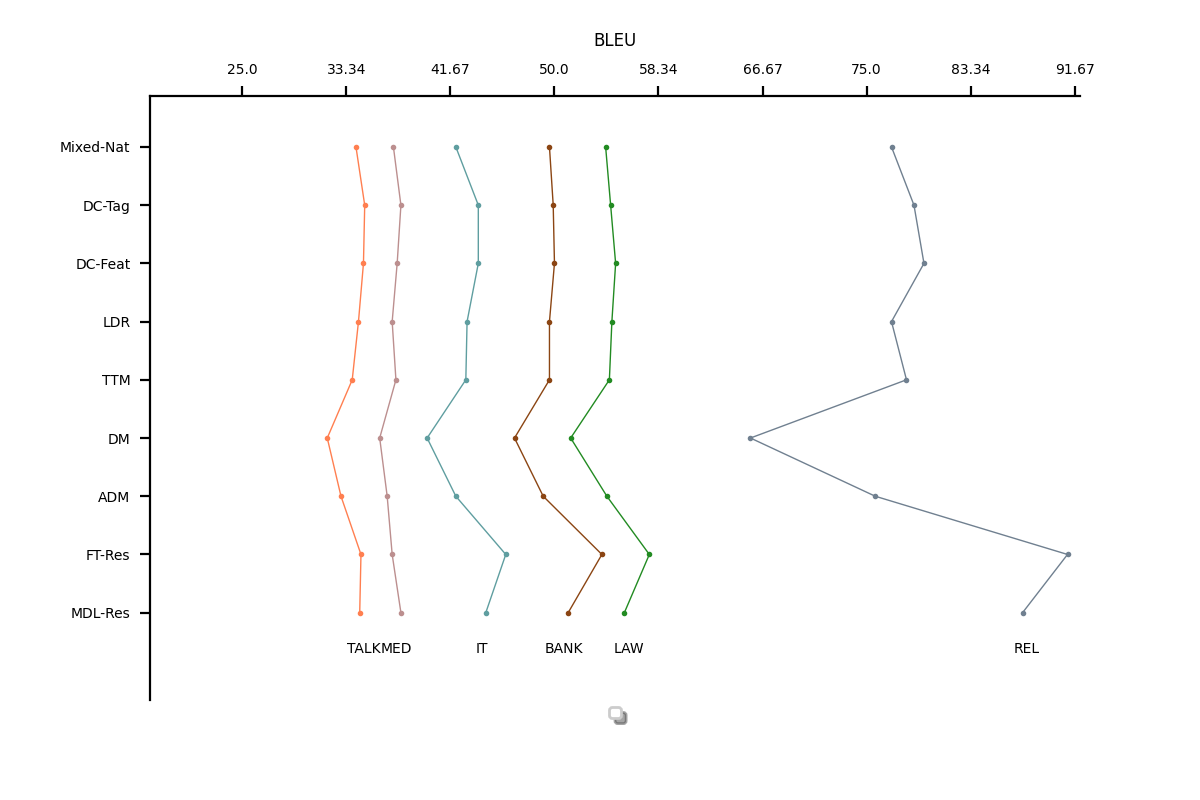
\includegraphics[width=\textwidth]{unbalanced.png}
\end{figure}
\end{frame}
%---------------------------------------------------------

%---------------------------------------------------------
\begin{frame}
\frametitle{OOD test set}
\begin{figure}
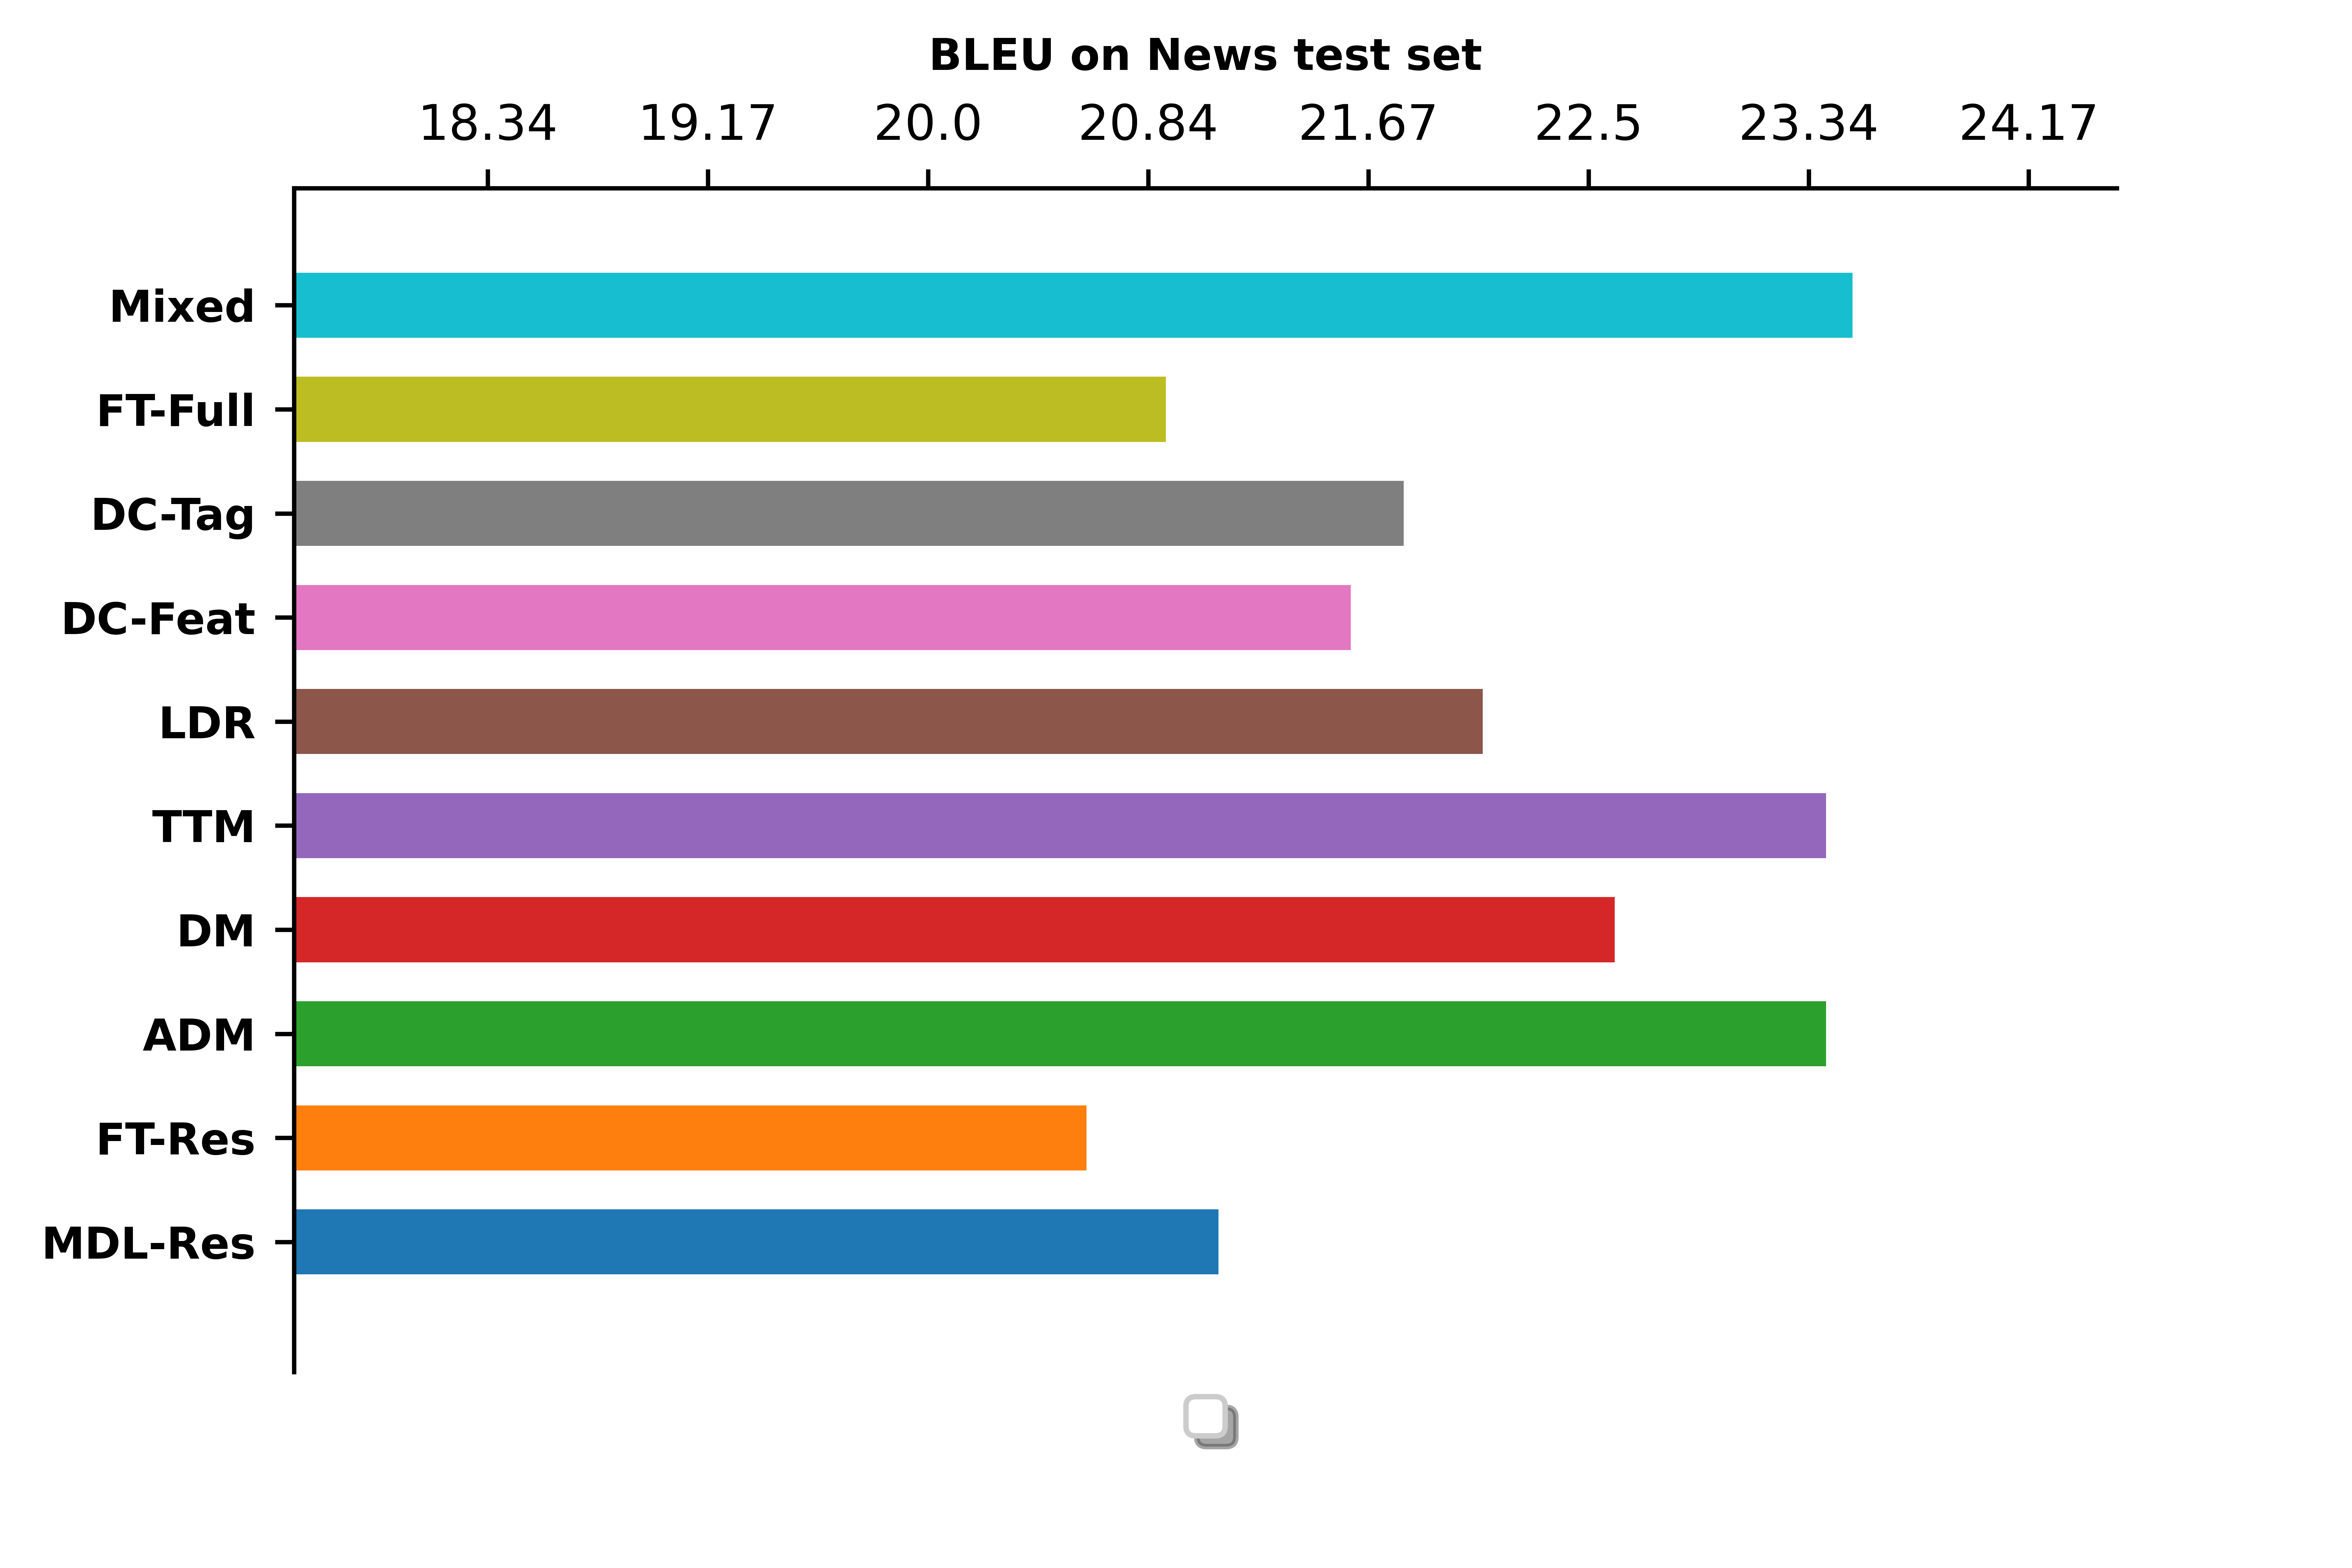
\includegraphics[width=\textwidth]{news.png}
\end{figure}
\end{frame}
%---------------------------------------------------------

%---------------------------------------------------------
\begin{frame}
\frametitle{Random tagged test set}
\begin{figure}
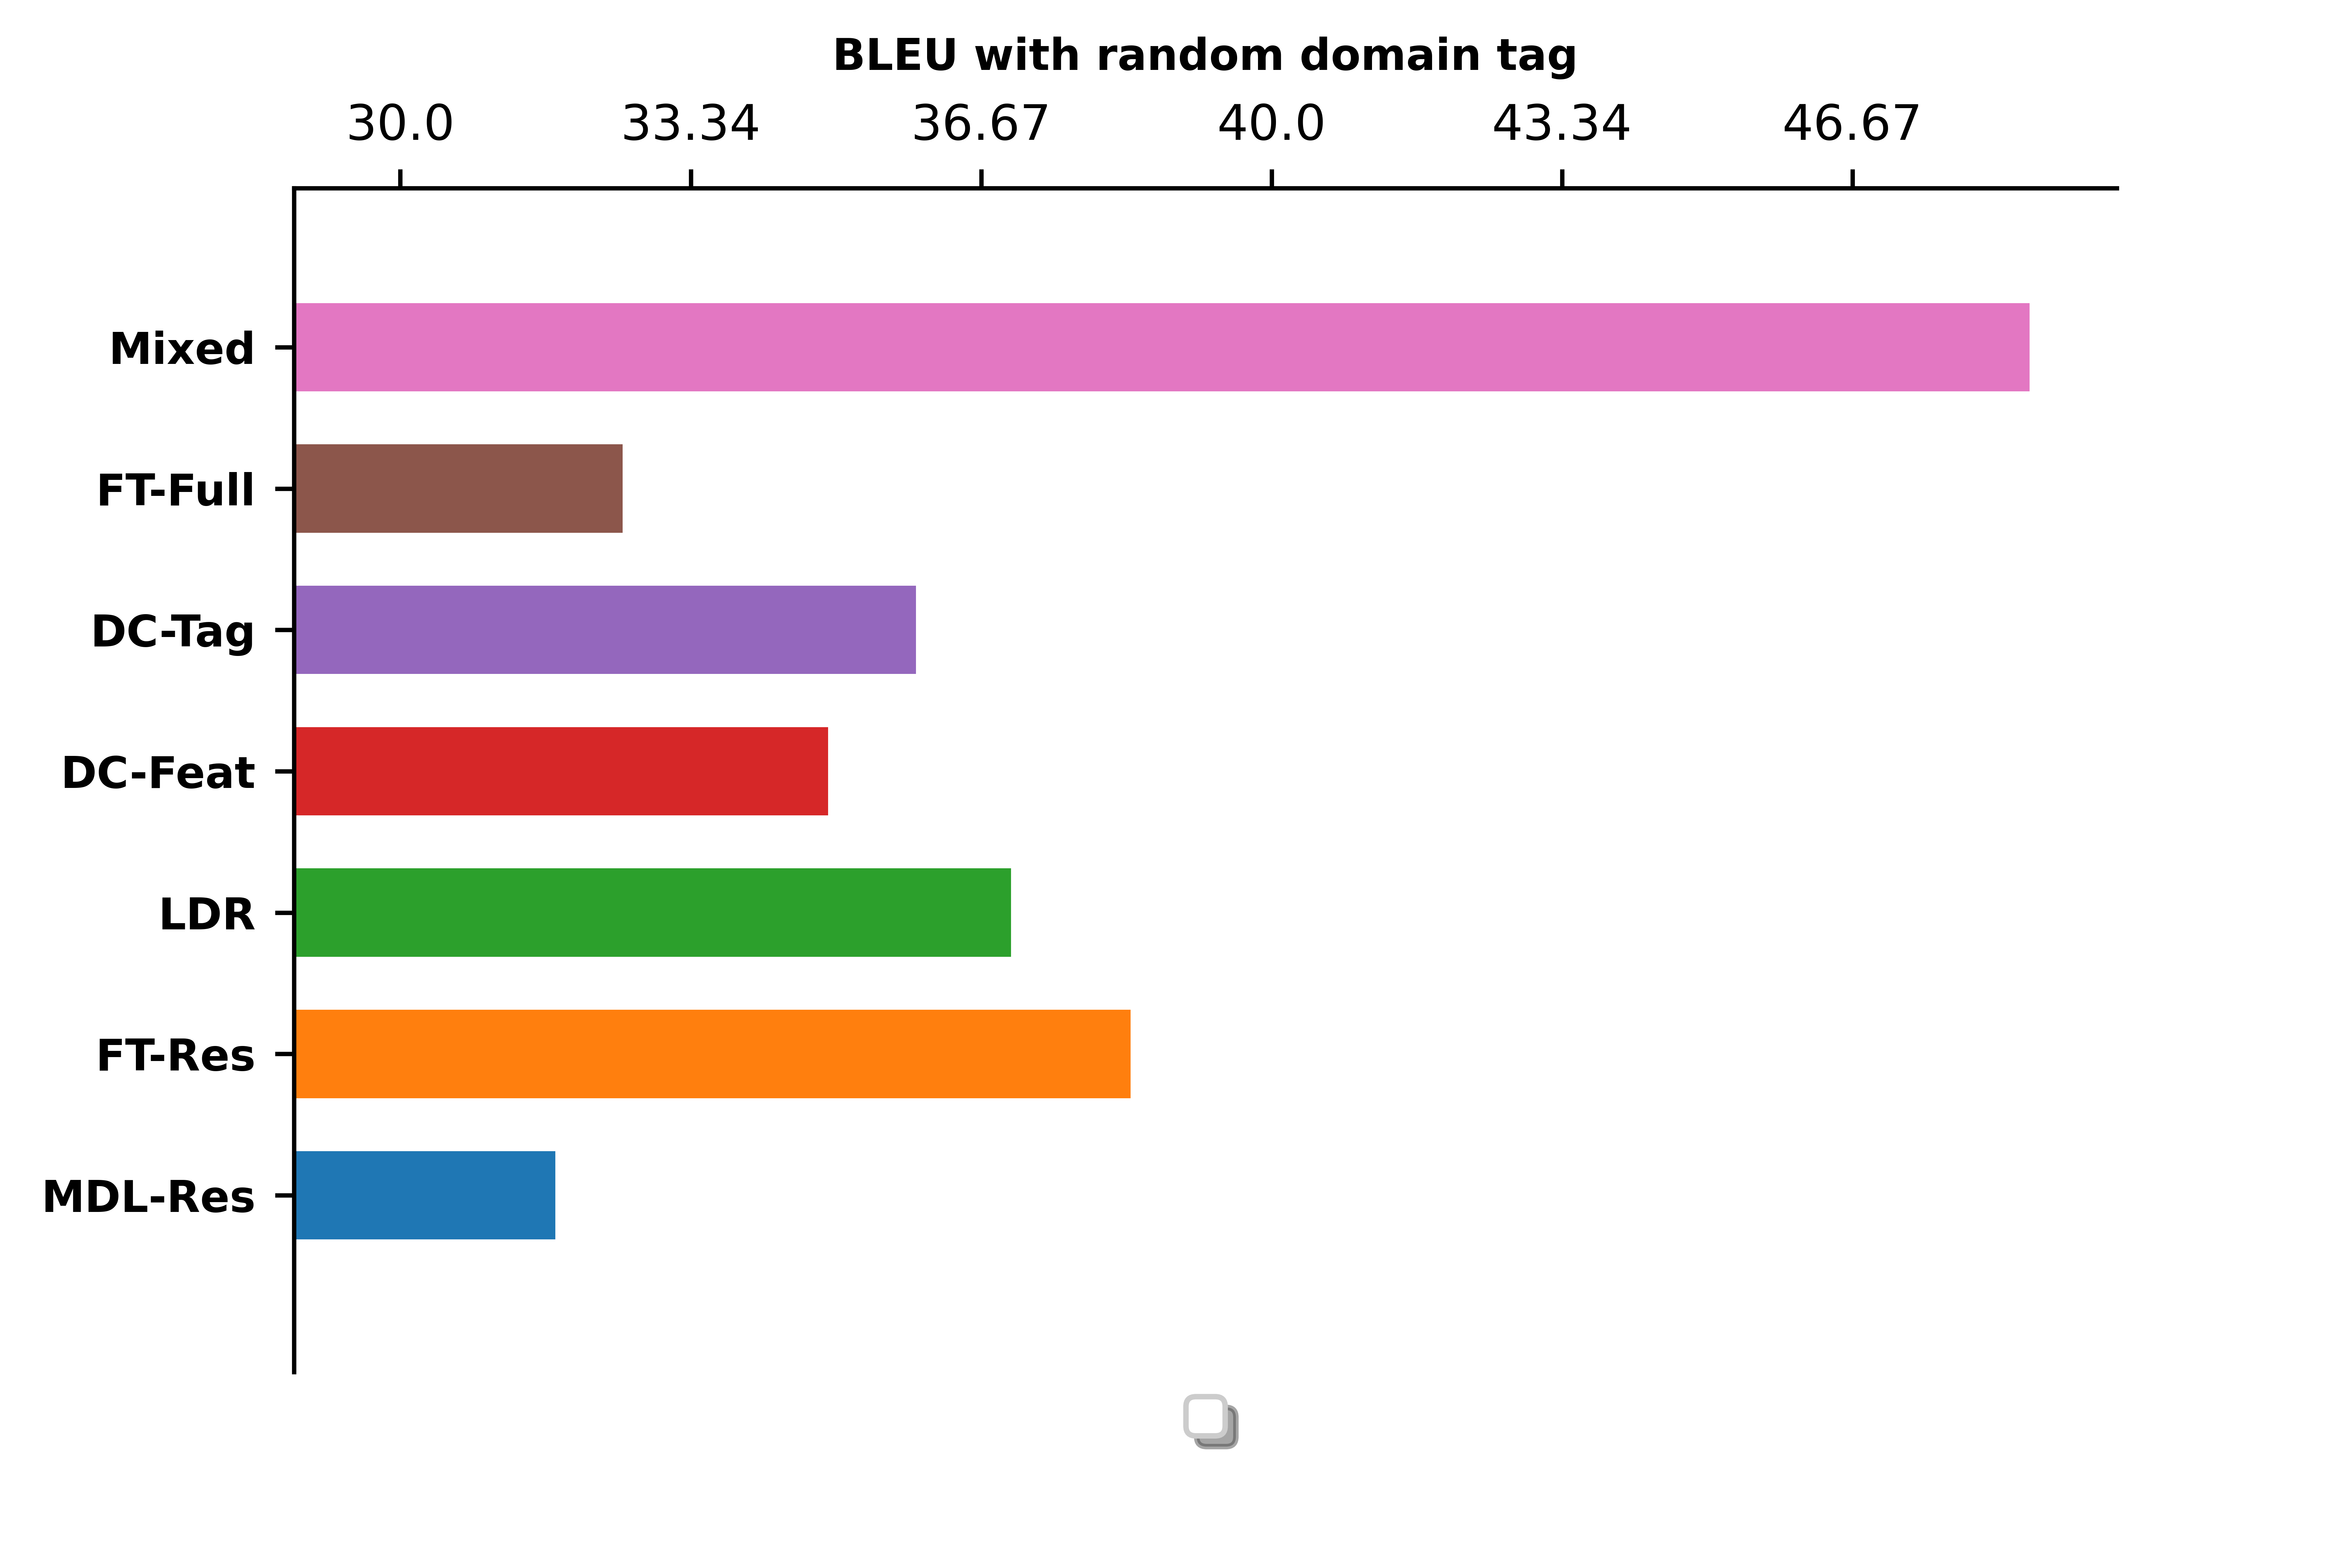
\includegraphics[width=\textwidth]{random_tag.png}
\end{figure}
\end{frame}
%---------------------------------------------------------

%---------------------------------------------------------
\begin{frame}
\frametitle{Fuzzy domain separation}
\begin{figure}
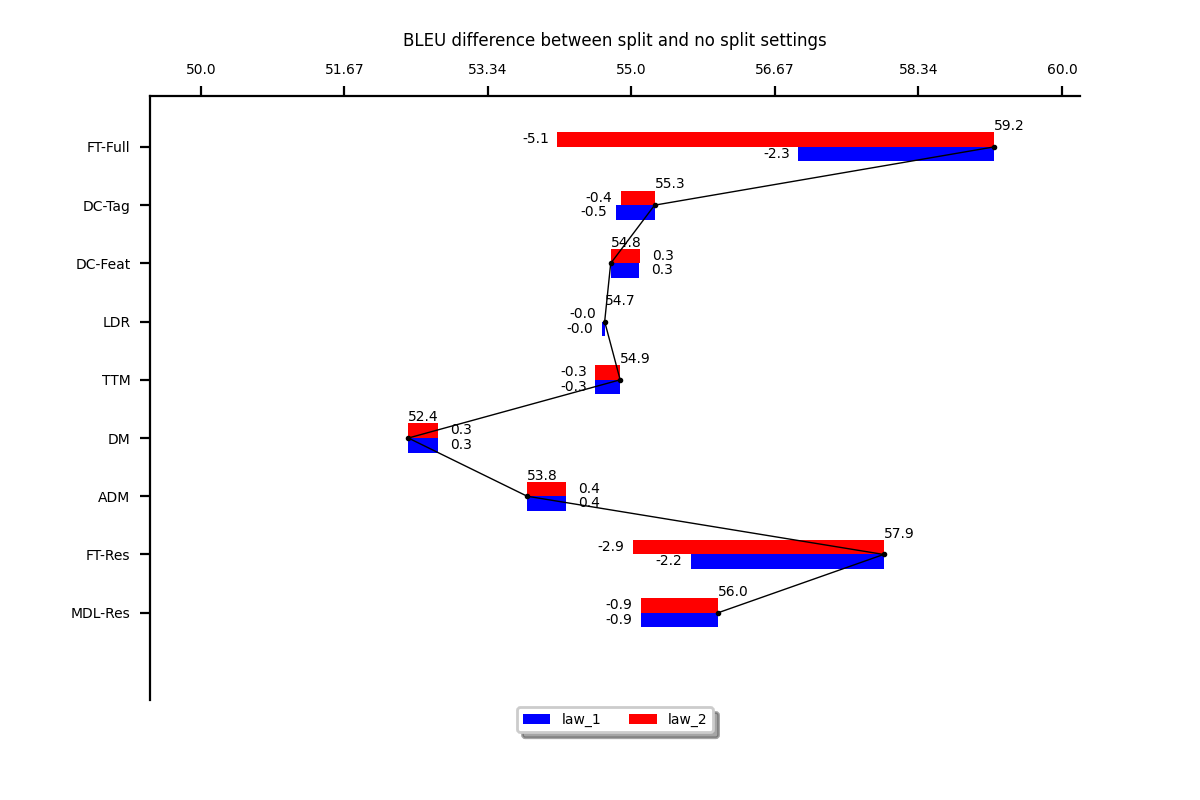
\includegraphics[width=\textwidth]{fuzzy_split.png}
\end{figure}
\end{frame}
%---------------------------------------------------------

%---------------------------------------------------------
\begin{frame}
\frametitle{Automatic clustering}
\begin{figure}
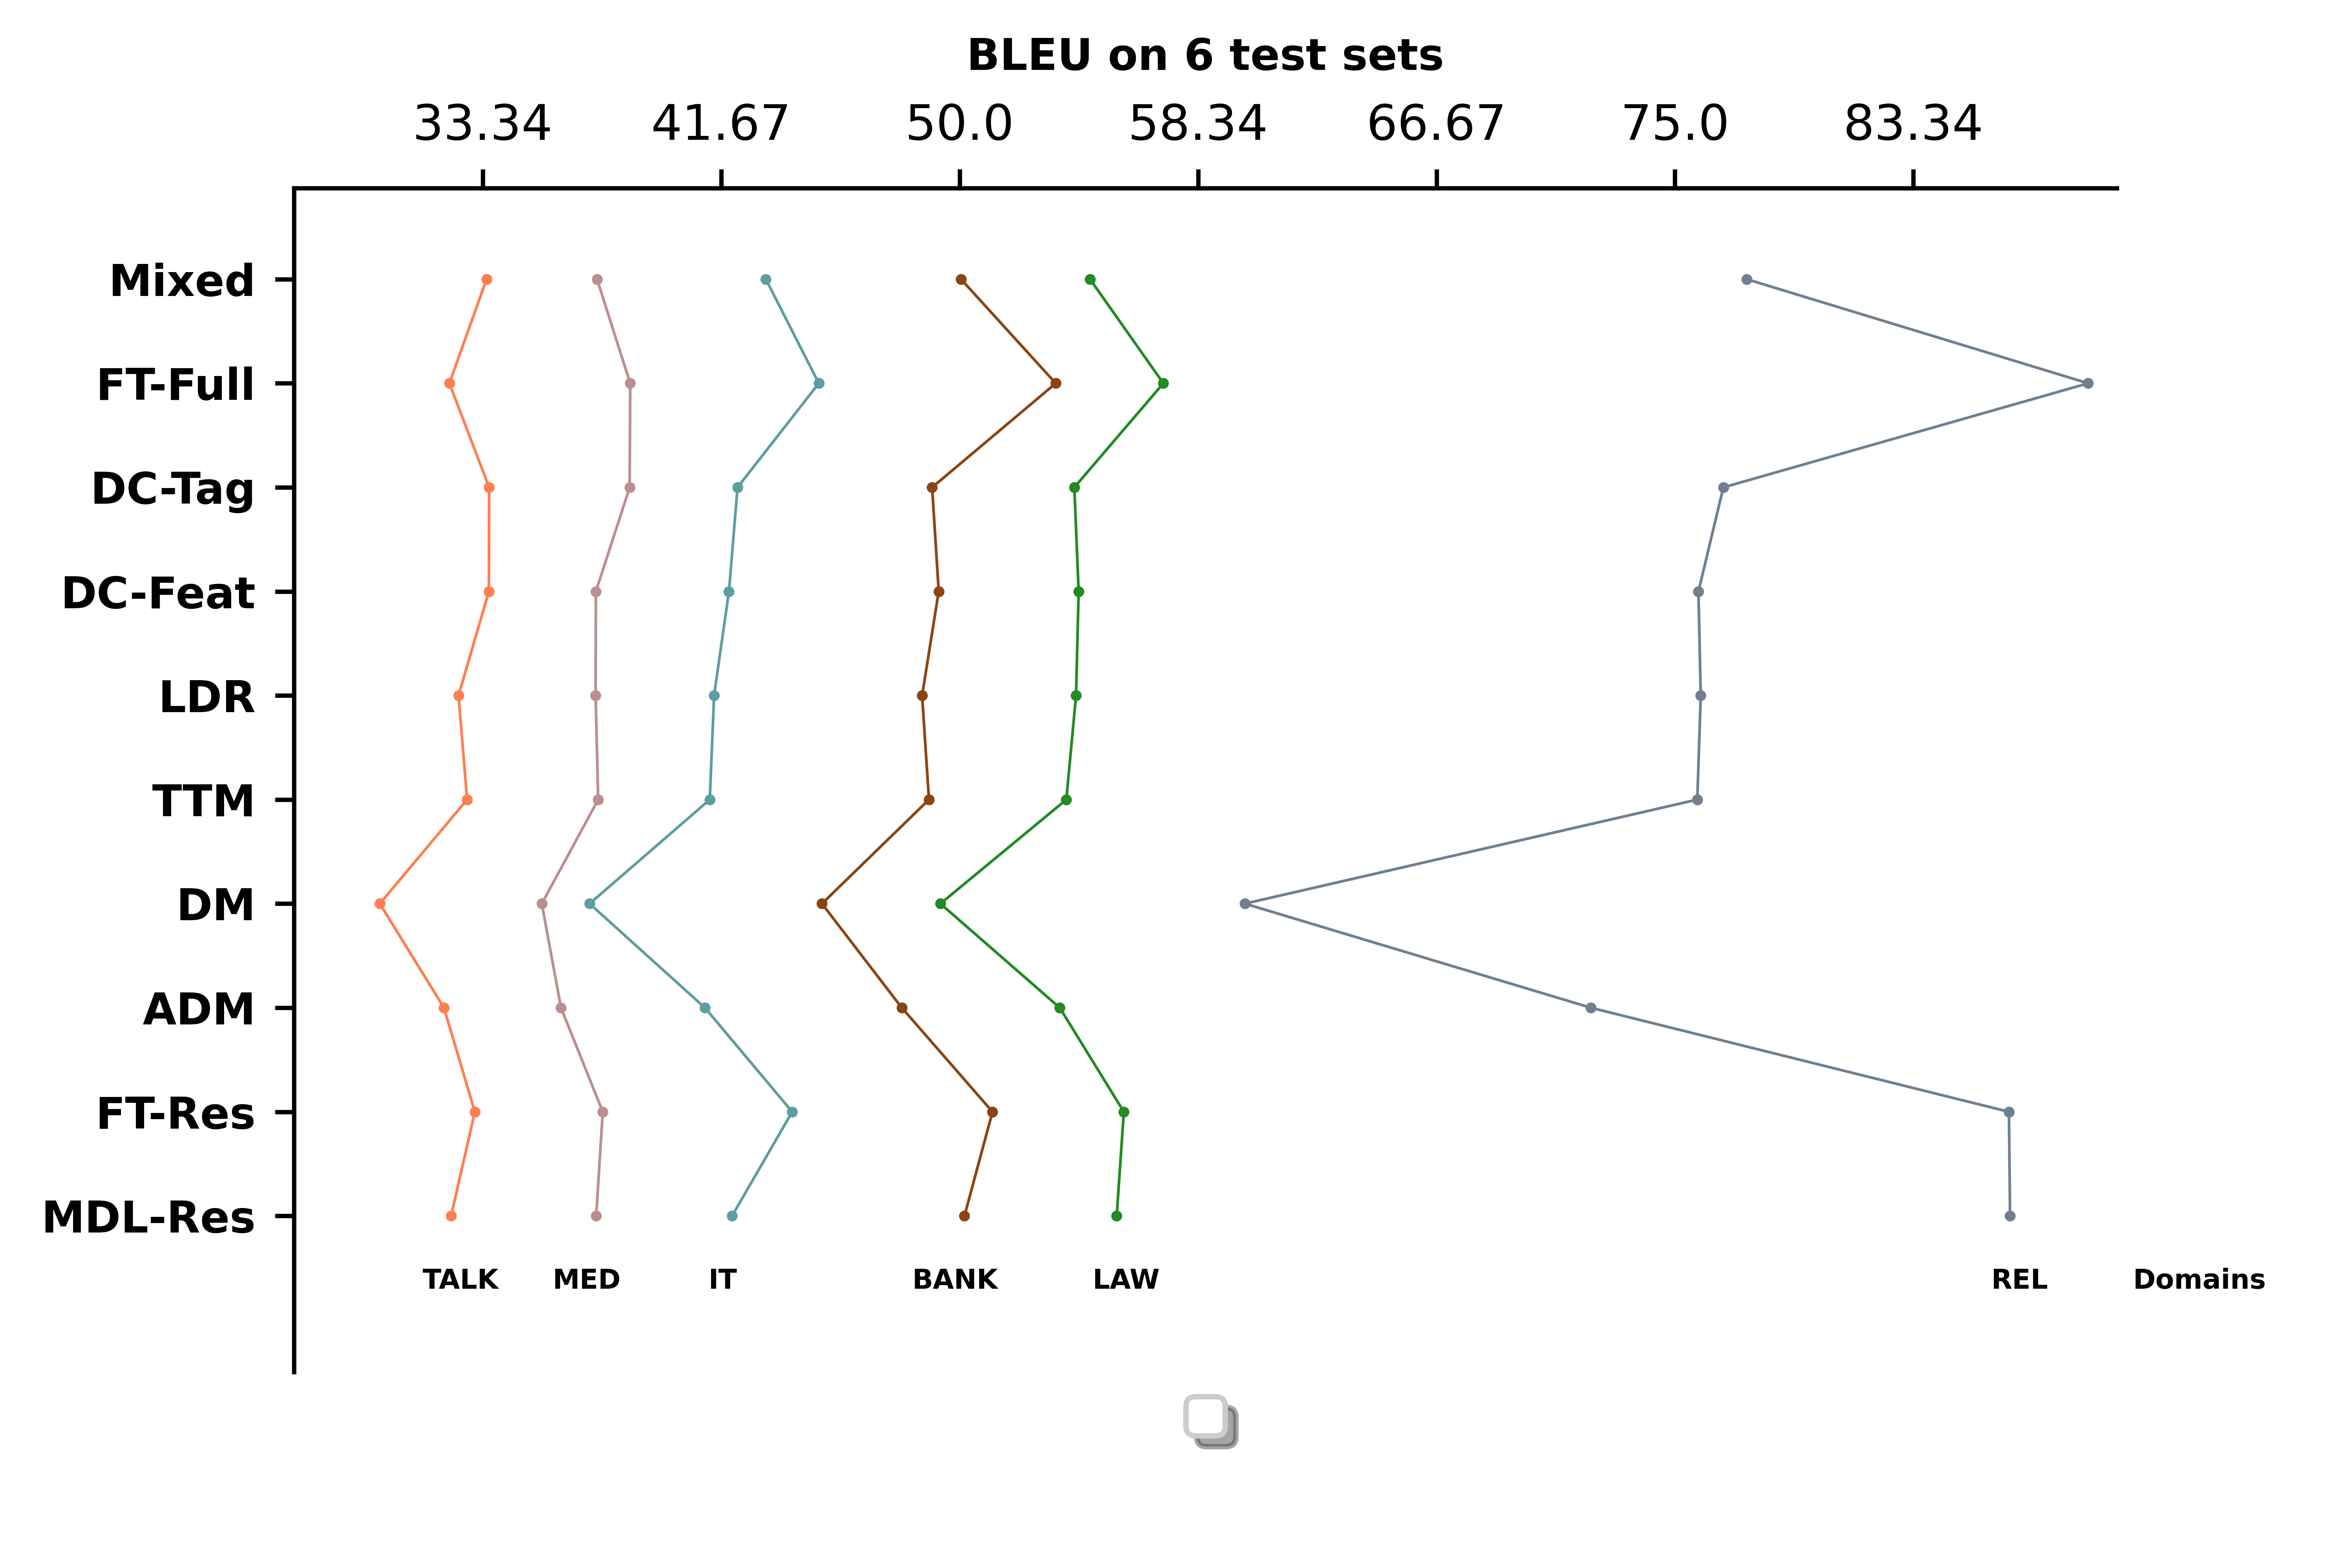
\includegraphics[width=\textwidth]{auto_cluster.png}
\end{figure}
\end{frame}
%---------------------------------------------------------

%---------------------------------------------------------
\begin{frame}
\frametitle{Continuous training}
\begin{figure}
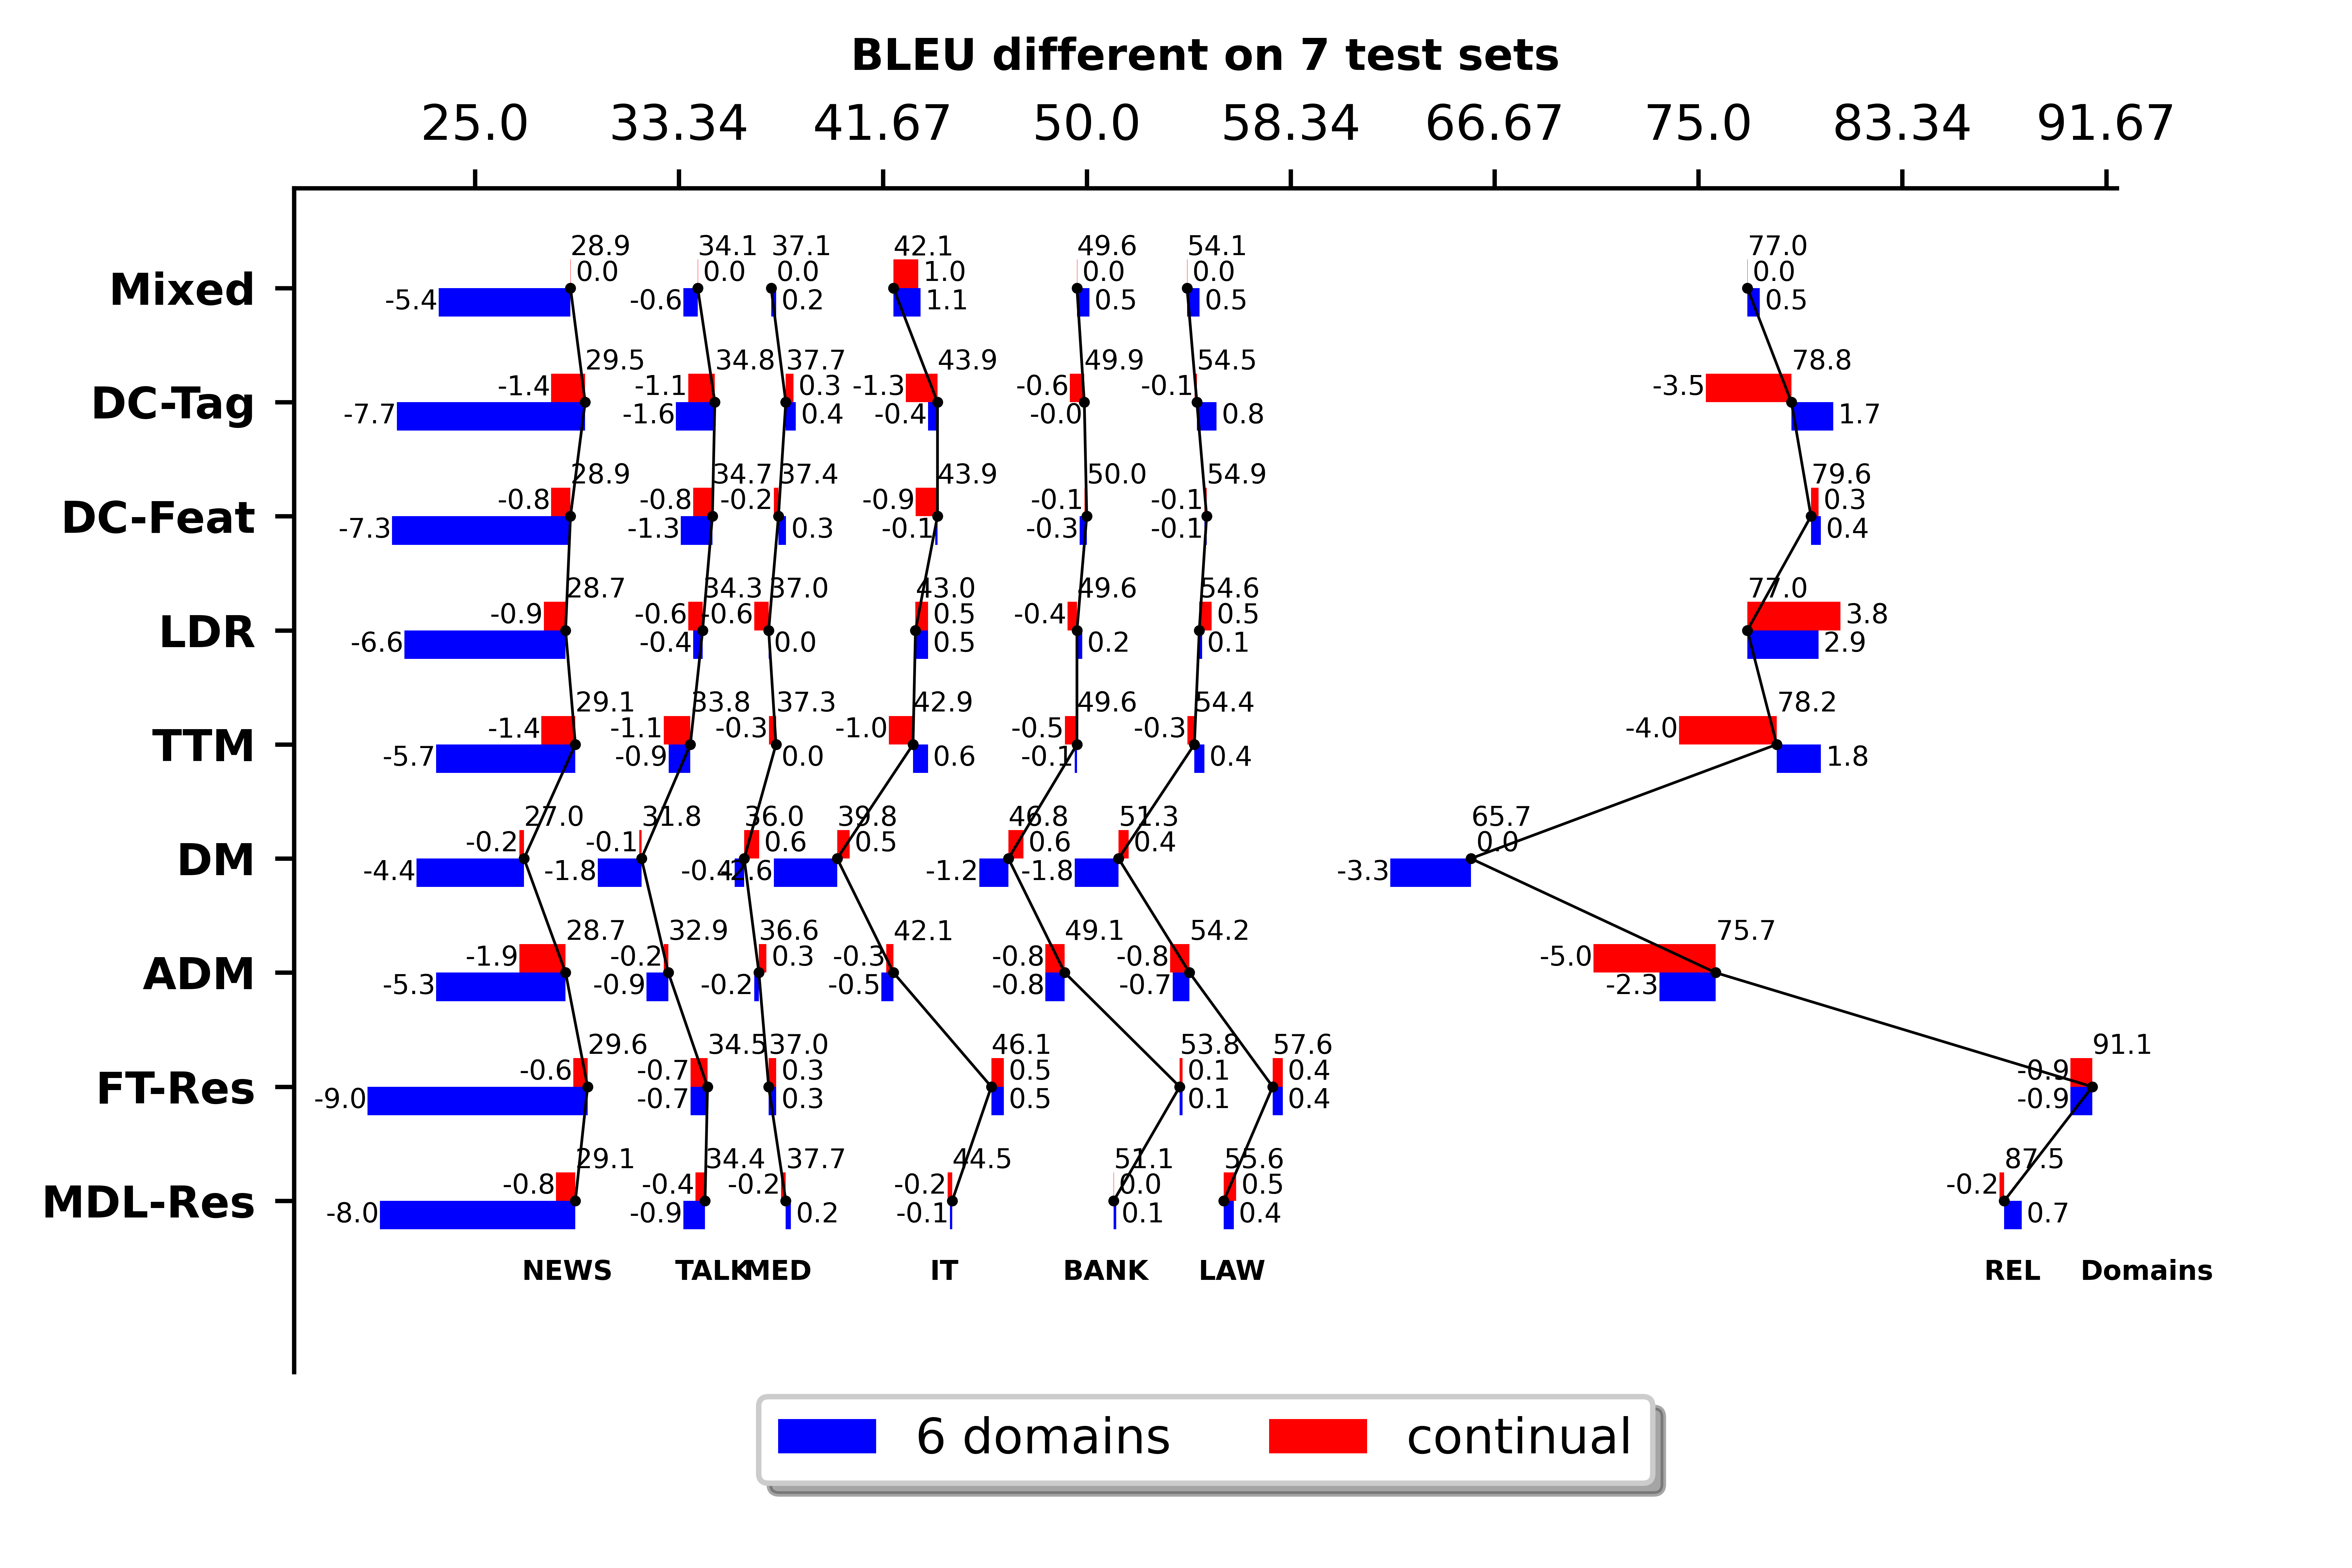
\includegraphics[width=\textwidth]{continuous_training.png}
\end{figure}
\end{frame}
%---------------------------------------------------------

%%%%%%%%%%%%%%%%%%%%%%%%%%%%%%%%%%%%%%%%%%%%%%%%%%%%%%%%%%
\section{Discussion} %%%%%%%%%%%%%%%%%%%%%%%%%
%%%%%%%%%%%%%%%%%%%%%%%%%%%%%%%%%%%%%%%%%%%%%%%%%%%%%%%%%%

%---------------------------------------------------------
%Two columns
\begin{frame}
\begin{itemize}
	\item Multi-domain NMT is a hard problem that requires much more effort of research.
	\item The standard evaluation, which is often reported in the papers working on multi-domain NMT, is naive.
	\item A call for building robust NMT systems in more realistic scenarios: \newline
          eg.\ large number of domains, extreme unbalancing, unseen domains and continuous learning etc.
	\item \fyTodo{To add more conclusions}
	
\end{itemize}
\end{frame}
%---------------------------------------------------------

%---------------------------------------------------------
\begin{frame}

\centering
\Huge
Thank you \\
\vspace{1.5cm}
    
\includegraphics[height=1.0cm]{systran-logo.png}
    
\includegraphics[height=1.0cm]{cnrs-logo.png}
%    
\includegraphics[height=1.0cm]{limsi-logo.png}
    
\includegraphics[height=1.0cm]{ups-logo.png}
\end{frame}
%---------------------------------------------------------

\bibliography{multidomain}

\end{document}